\documentclass{JNUexp}
\courseName{计算机图形学}
\expName{实验 5 实体造型和纹理映射}
\expDate{2017.12.7}
\className{计科1404}
\studentName{阎覃}
\studentId{1030414414}

\graphicspath{ {images/} }

\usepackage[hidelinks]{hyperref}
\usepackage{amsmath}
\begin{document} 

\section{实验内容}
设计并实现一个针对简单3D物体的实体造型算法,实现纹理映射算法。

\section{实验步骤及运行情况}
%%%%%%%%%%%%%%%%%%%%%%%%%%%%%%%%%%%%%%%%%%%%%%%%%%%%%%%%%%%%%%%%%%%%%%%%%%%%%%%%
%   1 设计并实现一个针对简单3D物体的实体造型算法,实现纹理映射算法。
%%%%%%%%%%%%%%%%%%%%%%%%%%%%%%%%%%%%%%%%%%%%%%%%%%%%%%%%%%%%%%%%%%%%%%%%%%%%%%%%
\begin{problem}
    设计并实现一个针对简单3D物体的实体造型算法,实现纹理映射算法。
\end{problem}

\begin{answer}
以下代码实现了绘制长方体的实体造型和纹理映射的算法。

完整程序在本文最后的网址中。

    \begin{lstlisting}[language=C++]
// 绘制长方体 width,height,depth分别为长方体的长,高和深度
void DrawCube(GLfloat width, GLfloat height, GLfloat depth) {
    GLfloat x = width / 2, y = height / 2, z = depth / 2;

    glBegin(GL_QUADS);
    // 前面(front)
    glBindTexture(GL_TEXTURE_2D, texture->id);
    glNormal3f(0, 0, 1);
    glTexCoord2f(0, 0);
    glVertex3f(-x, -y, z);
    glTexCoord2f(1, 0);
    glVertex3f(x, -y, z);
    glTexCoord2f(1, 1);
    glVertex3f(x, y, z);
    glTexCoord2f(0, 1);
    glVertex3f(-x, y, z);
    // 背面(back)

    glNormal3f(0, 0, -1);
    glTexCoord2f(0, 0);
    glVertex3f(x, -y, -z);
    glTexCoord2f(1, 0);
    glVertex3f(-x, -y, -z);
    glTexCoord2f(1, 1);
    glVertex3f(-x, y, -z);
    glTexCoord2f(0, 1);
    glVertex3f(x, y, -z);

    // 右侧面(right)
    glNormal3f(1, 0, 0);
    glTexCoord2f(0, 0);
    glVertex3f(x, -y, z);
    glTexCoord2f(1, 0);
    glVertex3f(x, -y, -z);
    glTexCoord2f(1, 1);
    glVertex3f(x, y, -z);
    glTexCoord2f(0, 1);
    glVertex3f(x, y, z);
    // 左侧面(left)
    glNormal3f(-1, 0, 0);
    glTexCoord2f(0, 0);
    glVertex3f(-x, -y, -z);
    glTexCoord2f(1, 0);
    glVertex3f(-x, -y, z);
    glTexCoord2f(1, 1);
    glVertex3f(-x, y, z);
    glTexCoord2f(0, 1);
    glVertex3f(-x, y, -z);

    // 顶面(top)
    glNormal3f(0, 1, 0);
    glTexCoord2f(0, 0);
    glVertex3f(-x, y, z);
    glTexCoord2f(1, 0);
    glVertex3f(x, y, z);
    glTexCoord2f(1, 1);
    glVertex3f(x, y, -z);
    glTexCoord2f(0, 1);
    glVertex3f(-x, y, -z);
    // 底面(bottom)
    glNormal3f(0, -1, 0);
    glTexCoord2f(0, 0);
    glVertex3f(-x, -y, -z);
    glTexCoord2f(1, 0);
    glVertex3f(x, -y, -z);
    glTexCoord2f(1, 1);
    glVertex3f(x, -y, z);
    glTexCoord2f(0, 1);
    glVertex3f(-x, -y, z);
    glEnd();
}

    \end{lstlisting}
\end{answer}

\begin{image}
    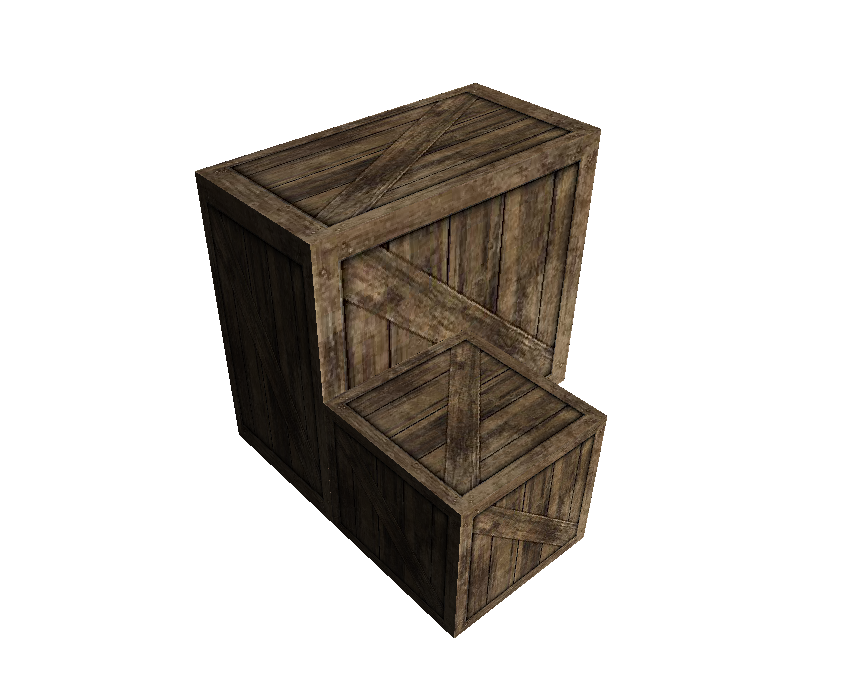
\includegraphics[width=0.7\textwidth]{1}
\end{image}

\newpage
\section{实验体会}
本次试验实现了一个简易的实体造型算法,再结合之前的3D变换,绘制了两个会旋转的箱子。为了更逼真我在网上搜索了木箱子的材质图片,使用OpenCV和OpenGL,实现了纹理映射。

\vfill

实验报告采用 \LaTeX 排版,完整代码托管至GitHub:\\
\url{https://github.com/Ethan-yt/JNU-CG-exp}

\end{document}